% !TeX spellcheck = fr_FR
\chapter{Chapitre 3 : Méthodologie}

\section{Machine learning}

Tout d'abord revennons sur les technologies de bases sur lequel ce projet se porte. 
Dans ce projet, nous avons essayer de créer un programme capable d'analyser un signal temporel et 
d'en estimer la présence et la quantité de photons présent dans ce signal.

Pour cela, nous avons utilisés différents types de réseaux neuronaux qui sont eux-mêmes une technique de machine learning.
Le machine learning peut-être n'importe quel forme de programme ou système capable d'apprendre ou d'améliorer ses performances
en fonction des données qu'il traite.

Il existe deux types d'apprentissage pour le machine learning : supervisé et non supervisé.
Le premier signifie que les données utilisées pour entrainer un système contient aussi les conclusions qu'il doit en tirer.
Par exemple une image et un texte descriptif. Au fur et à mesure d'analyser ces diférentes données le système de machine learning
va donc y trouver des informations ou patterns auquel il va attribuer les conclusions prédéfinies.

Pour l'apprentissage non supervisé, le système de machine learning utilise des données brutes qui n'ont pas de conclusions ou descriptions associées.
Ce modèle va alors lui même essayer de trouver une manière de classifier ou donner un score sur ces données brutes.

Dans le cadre de ce projet, l'équipe de l'\gls{unige} nous a fournis des données provenant de simulations des capteurs conçus pour les différents télescopes analysés.
Lors de la création de ces simulations, les méta-données des photons simulés a aussi été sauvegardée, ce qui nous donne accès
à la "vérité" de la quantité et à quel moment les photons ont été détectés. 
Formalisant le but du projet comme : la recherche d'une architecture de réseau de neurones avec un apprentissage supervisée.

\section{Réseaux neuronaux}

Maintenant parlons de ce qu'est un réseau de neurones ou réseau neuronal.
Comme vu précédemment, c'est un modèle de machine learning qui est inspiré par le fonctionnement d'un cerveau humain.

%TODO insert neural network image here

Cette technique utilise des noeuds (neurones artificiels) interconnectés entre eux, créant ainsi des couches similiares à nos cerveaux.
Chaque noeud ou neurone peut être ou non connecté à un ou plusieurs suivants laissant une infinité d'interconnexions, 
cela peut aussi être surnommer comme l'architecture du réseau.

\subsection{Les perceptrons}

Le fonctionnement d'un neurone standard suis le fonctionnement suivant :

% TODO perceptron image

Celui-ci prend en entrée : un bias, et x données avec des poids associés. Toutes ces valeurs biasées sont ensuite additionnées ensemble
et passées à une fonction d'activation qui donnera une valeur de sortie au perceptron. 

Avec un seul perceptron, il est possible d'ajuster ces poids de telle manière à lui faire apprendre une motif de
séparation linéaire en fonction des données d'entrée. 

\begin{figure}[tbph!]
	\centering
	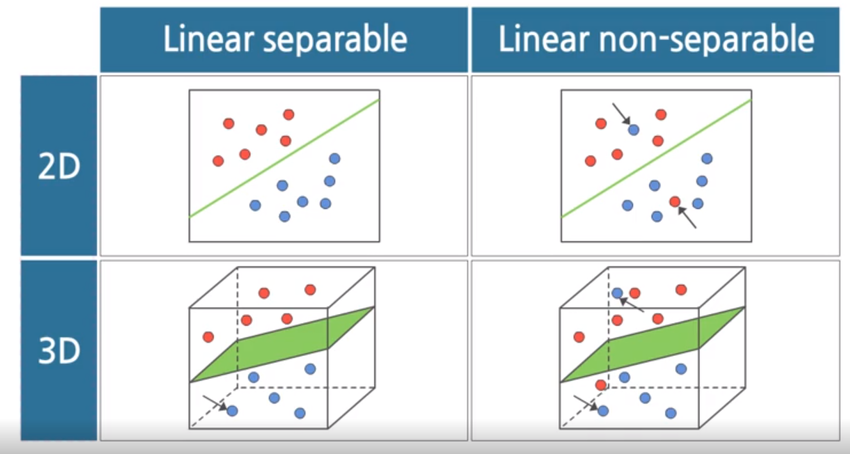
\includegraphics[width=0.4\linewidth]{separation-lineaire.png}
	\caption[Comparaison de données séparables ou non linéairement]{Comparaison de données séparables ou non linéairement. Source : \cite{LinearSeparation}}
\end{figure}

Il a donc été rapidement imaginé d'interconnecter ces perceptrons pour permettre d'apprendre des problèmes non linéaires.

\subsection{Multi Layer Perceptron}
L'architecture la plus simple de réseaux de neurones est de simplement connecter chaque couche de neurones entre eux.

%TODO MLP image




\section{Données}




% Au cours de ce projet, j'ai tester différentes configuration de réseau de neurones sur des données.
% Celles-ci sont des données provenant de simulation. Le premier simulateur que j'ai utilisé s'appelle

%%%%%%%%%%%%%%%%%%%%%% chap 2 maintenant
% \section{Remise en contexte}
% La problématique qui a lancé ce projet est la quantité limitée de bande passante de transmission à bord de Terzina. 
% La bande passante du satellite NUSES est partagée avec Zirè et limite donc Terzina à 40Gbit par jour en transmission et quelques Kbit en réception.
% Bien que les capteurs aient déjà un déclanchement matériel, celui-ci était jugé comme insuffisant par l'équipe de l'\gls{unige} pour filtrer 
% les évènements d'intérêt scientifique sans dépasser la limite de transmission.

% Il a donc été proposé de rajouter un réseau de neurones qui pourrait être capable de filtrer le bruit de chaque pixel pour n'en garder que 
% l'onde connue des photons de pluies atmosphériques. Avec ce signal filtré, une décision d'envoyer ou non l'évènement au sol
% serait plus simple. 

% Le réseau de neurones est prévu d'être programmé directement dans un \gls{fpga} pour des raisons d'optimisations de ressources à bord. 
% Le fait de déployer le modèle de réseau de neurones ne fait pas partie intégrante de ce travail mais implique une
% restriction technique car la programmation du \gls{fpga} ne sera possible qu'avant le lancement.
% De plus, les ressources à bord étant coûteuses, le modèle sera aussi conçu pour être le plus petit possible 
% afin d'utiliser le moins de place et de puissance de calcul.
% Il est prévu d'utiliser un modèle Keras pour le réseau de neurones, car il existe déjà des moyens de l'exporter vers des \gls{fpga}.

% En plus de cette utilisation en tant que filtre, il a été théorisé avec l'équipe de l'\gls{unige} que le réseau de neurones
% pourrait aussi compenser l'usure/l'irradiation des capteurs. Ceci pourrait être fait par un ajustement en vol des poids du réseau de neurones 
% ou par le fonctionnement du modèle lui-même.
%%%%%%%%%%%%%%%%%%%%%%%%%%

\section{Simulateurs d'onde}
Le début de mon projet a consisté à récupérer deux simulateurs de photomultiplicateurs et à m'acclimater à ce domaine de la physique.
Pendant toute la mise en place de ces simulateurs, j'ai aussi installé un environnement de développement avec les librairies Python et les drivers Nvidia.

\begin{figure}[tbph!]
	\centering
	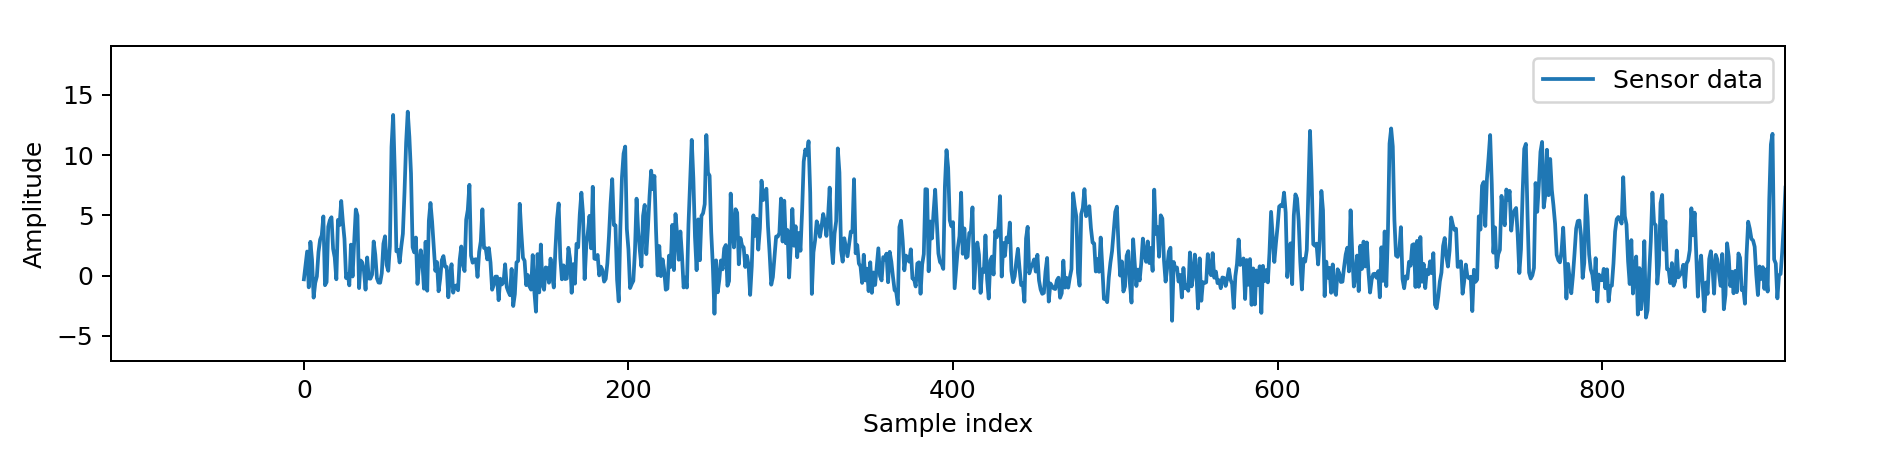
\includegraphics[width=\linewidth]{sensor_waveform.png}
	\caption[Exemple d'onde simulée]{Exemple d'onde simulée en sortie de capteur/ASIC.}
\end{figure}

Le premier : "terzina\_wfsim" est un simulateur développé en C/C++ qui génère des fichiers ROOT contenant l'onde en sortie du capteur.
Cependant, celui-ci s'est révélé limité très rapidement car les fichiers créés contiennent l'onde attendue combinée avec du bruit simulé,
mais la simulation d'un photon à haute énergie n'était faite qu'une seule fois au même endroit pour chaque onde.

Le deuxième : "pe\_extractor" \cite{PeExtractor} est un projet contenant un simulateur d'onde couplé à des tests de machine learning pour détection de \gls{pe} développé en Python.
Le concept de "photo électron" ou \gls{pe} est en réalité la charge électrique détectée par le capteur due à une interaction avec un photon dans le photomultiplicateur.
Ce projet ne partageant pas les mêmes problèmes de génération de données que le précédant et étant capable de générer des données en continu dans des programmes Python,
nous avons préféré concentrer nos efforts sur celui-ci.

Les premières semaines de ce travail ont été dédiées à faire fonctionner ce générateur ainsi qu'à analyser son fonctionnement et ses paramètres.
Il fonctionne en simulant du bruit et en y rajoutant des interactions électriques par un fichier d'impulsion modèle. 
Le générateur va nous fournir deux tableaux en sortie : le signal discrétisé et des bacs contenant la vérité du nombre de \gls{pe} ayant été injectés sur cette période.

Voici les paramètres importants du générateur et leur explication :
\begin{enumerate}
    \item "pe\_rate\_mhz" : Définit la fréquence moyenne à laquelle un \gls{pe} est injecté dans le signal.
        L'injection de \gls{pe} est aléatoire en suivant une distribution Poisson.
    \item "sampling\_rate\_mhz" : Définit la vitesse d'échantillonnage du signal. Pour Terzina, cela est de 200MHz.
    \item "n\_sample" et "n\_sample\_init" : Le générateur a un mécanisme d'initialisation pour le bruit électrique 
        qui peut prendre un certain nombre de cycles pour commencer a créer des informations cohérentes au niveau physique, 
        ces deux paramètres peuvent donc contrôler un nombre d'échantillons à écarter au début de la génération.
    \item "bin\_size\_ns" : Ce paramètre gère la période de comptabilisation des \gls{pe} insérés dans le signal de sortie.
    \item "shift\_proba\_bin" : Permet de décaler la comptabilisation de l'insertion de signal par un certain nombre de bacs.
        Ce système existe car l'impulsion a un temps de montée avant d'atteindre son pic, cela permet de décaler les bacs 
        de vérité pour s'aligner avec le pic de l'impulsion.
    \item "sigma\_smooth\_pe\_ns" : Ce paramètre sert à répartir le compte des \gls{pe} insérés sur les bacs voisines en ns
        pour éviter une vérité entière. 
    \item "noise\_lsb" : Est une quantité de bruit électronique.
\end{enumerate}

\section{Architectures envisagées}
Lors de nos premiers échanges, trois types de réseaux de neurones étaient envisagés pour répondre aux attentes de ce projet :

\subsection{Auto-encodeur}
L'auto-encodeur est une architecture de réseau de neurones particulière qui comprend deux parties distinctes d'encodage et de décodage. 
Ces deux étapes peuvent aussi être perçues comme une compression et décompression successive. \cite{IbmAutoencoder}

\begin{figure}[tbph!]
	\centering
	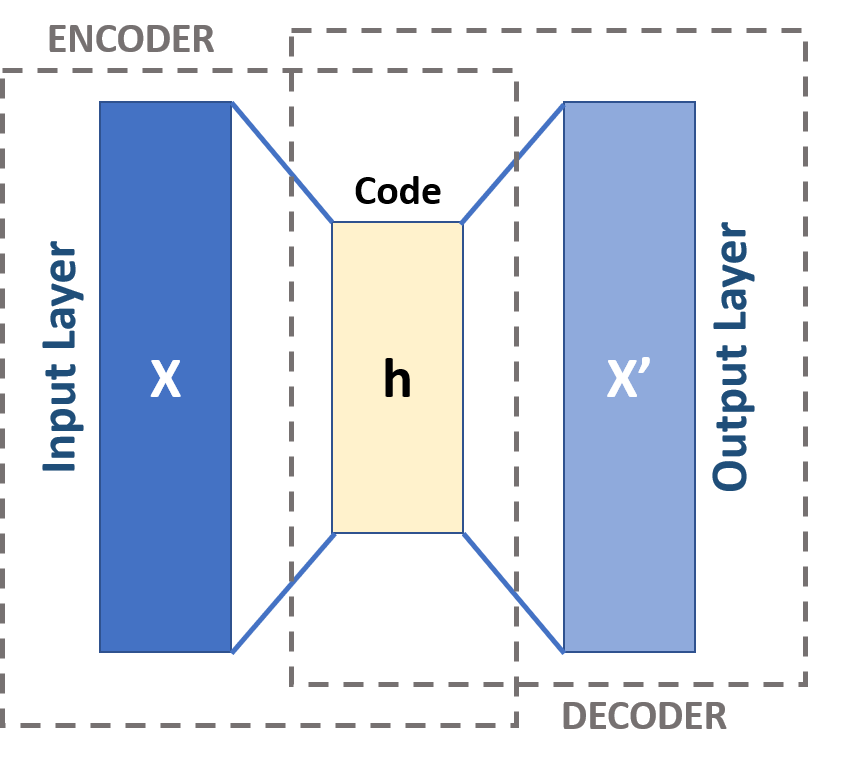
\includegraphics[width=0.4\linewidth]{Autoencoder.png}
	\caption[Schéma d'auto-encodeur]{Schéma d'auto-encodeur. Source : \cite{Autoencoder}}
\end{figure}

En entraînant le réseau de neurones, celui-ci va apprendre à réduire les informations en entrée jusqu'à un minimum pour 
ensuite essayer de reproduire au mieux les données originales à partir de cette représentation réduite.

Ce type de réseau pourrait bien fonctionner pour compresser les données des capteurs afin de les transmettre de manière compressée jusqu'au sol.
Cependant le fonctionnement des auto-encodeurs implique généralement une perte de précision notable lors de l'encodage des données.
Cela pourrait ne pas être un problème en soi pour la détection de la lumière Cherenkov. Cependant il est ressorti lors de nos réunions
une envie de garder des données plus près de celles en sortie des \gls{asic}, surtout pour la première mission qu'est Terzina.

\subsection{Réseau de neurones récurrents}
Un autre type de réseau neuronal que nous avions envisagé est le réseau de neurones récurrents. Cette architecture est adaptée
à des problèmes comprenant des données séquentielles ou temporelles généralement comme de la détection automatique de parole ou de texte.

Cette architecture diffère des autres réseaux de neurones car elle contient un mécanisme de "mémoire" intégré dans le modèle.
La mémoire est généralement implémentée en connectant la dernière sortie du modèle comme une entrée supplémentaire.

\begin{figure}[tbph!]
	\centering
	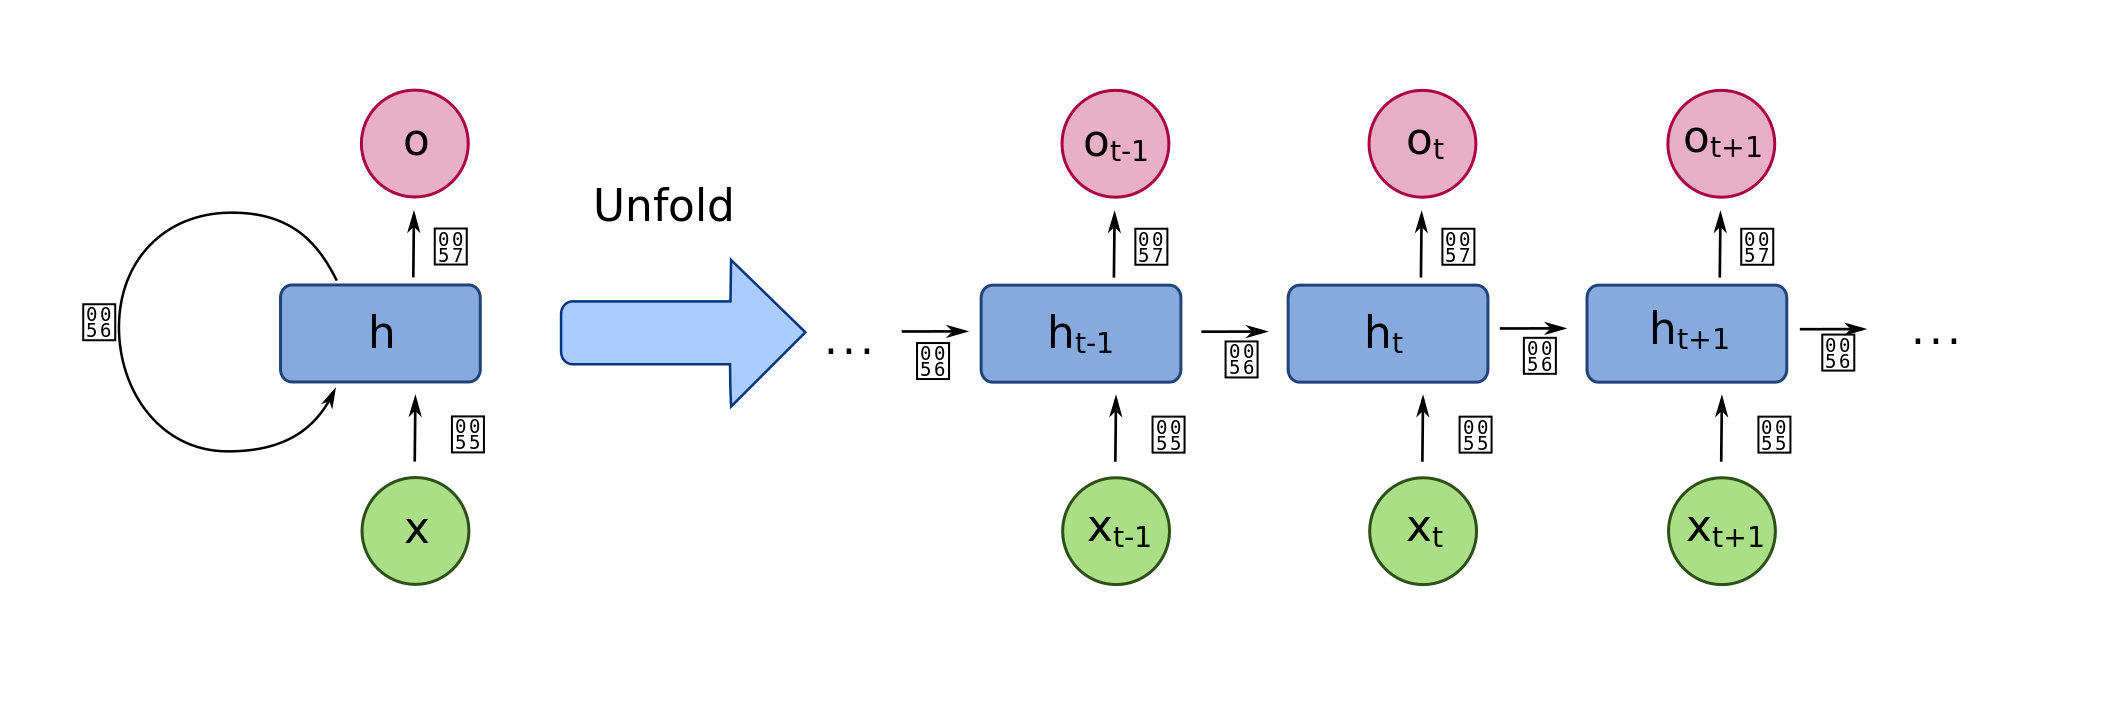
\includegraphics[width=0.4\linewidth]{rnn.png}
	\caption[Illustration de réseau de neurones récurrents]{Illustration de réseau de neurones récurrents. Source : \cite{RnnImage}}
\end{figure}

% Ce type de réseau serait le mieux adapté à un flux de données continues mais les \gls{asic} et leur déclencheur matériel
% ne fournissent que des fenêtres d'un certain nombre d'échantillons dans un laps de temps connu. 
% Bien qu'un RNN puisse fonctionner avec des fenêtres, cela nous paraissait contre-productif.

\subsection{Réseau de neurones convolutif}
L'architecture d'un réseau convolutif est semblable à un réseau de neurones standard a quelques exceptions près.
Dans un réseau de neurones standard, chaque neurone est connecté à chaque autre neurone des couches adjacentes;
dans le cas d'un réseau de neurones convolutif, certaines couches sont connectée d'une manière spécifique qui,
lorsqu'elle sera calculée, effectuera le même calcul qu'une convolution.

\begin{figure}[tbph!]
	\centering
	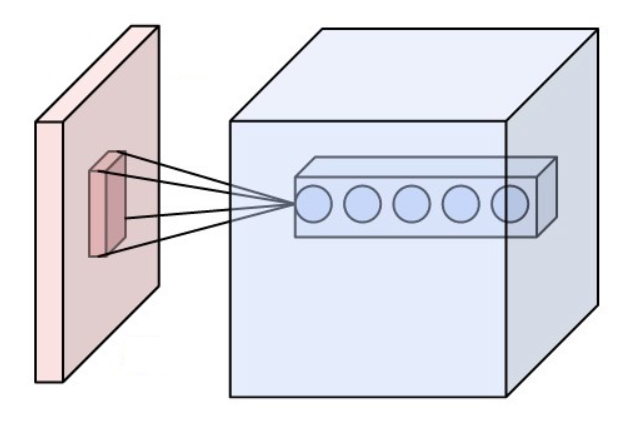
\includegraphics[width=0.4\linewidth]{Conv_layer.png}
	\caption[Illustration d'une couche convolutive de réseau neuronal]{Illustration d'une couche convolutive de réseau neuronal. Source : \cite{ConvImage}}
\end{figure}

L'opération de convolution en mathématique permet généralement d'extraire des informations d'une image comme le taux de 
variation d'intensité entre chaque pixel lors d'une détection de contours par exemple.
Ici, la différence est que le noyau utilisé pour la convolution n'est pas un noyau provenant d'algorithmes comme Sobel ou Canny mais c'est à nouveau
l'apprentissage du réseau qui va établir un noyau le plus optimisé pour trouver les caractéristiques recherchées dans les données d'entrée.

Dans le cadre de Terzina, c'est l'approche que nous avons privilégiée de par sa simplicité et le peu de resources qu'elle utilise.

%%%%%%%%%%%%%%%%% Chap 2 maintenant
% \section{Terzina - Retards de production}
% En mars dernier, lors de rendez-vous de coordination pour le projet Terzina, un retard conséquent sur la production des \gls{asic} prévus pour les capteurs à été révélé.
% Il a donc été décidé de remplacer ces \gls{asic} par un modèle déjà existant : CITIROC. Cependant, ces nouveaux \gls{asic} ne sont pas capables de transmettre une 
% onde comme les \gls{asic} prévus jusqu'à présent.
% Cet imprévu rend donc l'utilisation d'un réseau de neurones impossible à bord de Terzina. Cependant, il est encore intéressant de développer 
% ce modèle pour une utilisation dans de futurs satellites qui succèderont à Terzina. 

% J'ai donc été introduit au projet CTLearn et l'environnement qui l'entoure. 
% Ce projet est entre autre conçu pour classifier des pluies de lumière Cherenkov, 
% et pourrait possiblement bénéficier d'une étape de pré-traitement par pixels comme pour Terzina.

% \begin{figure}[tbph!]
% 	\centering
% 	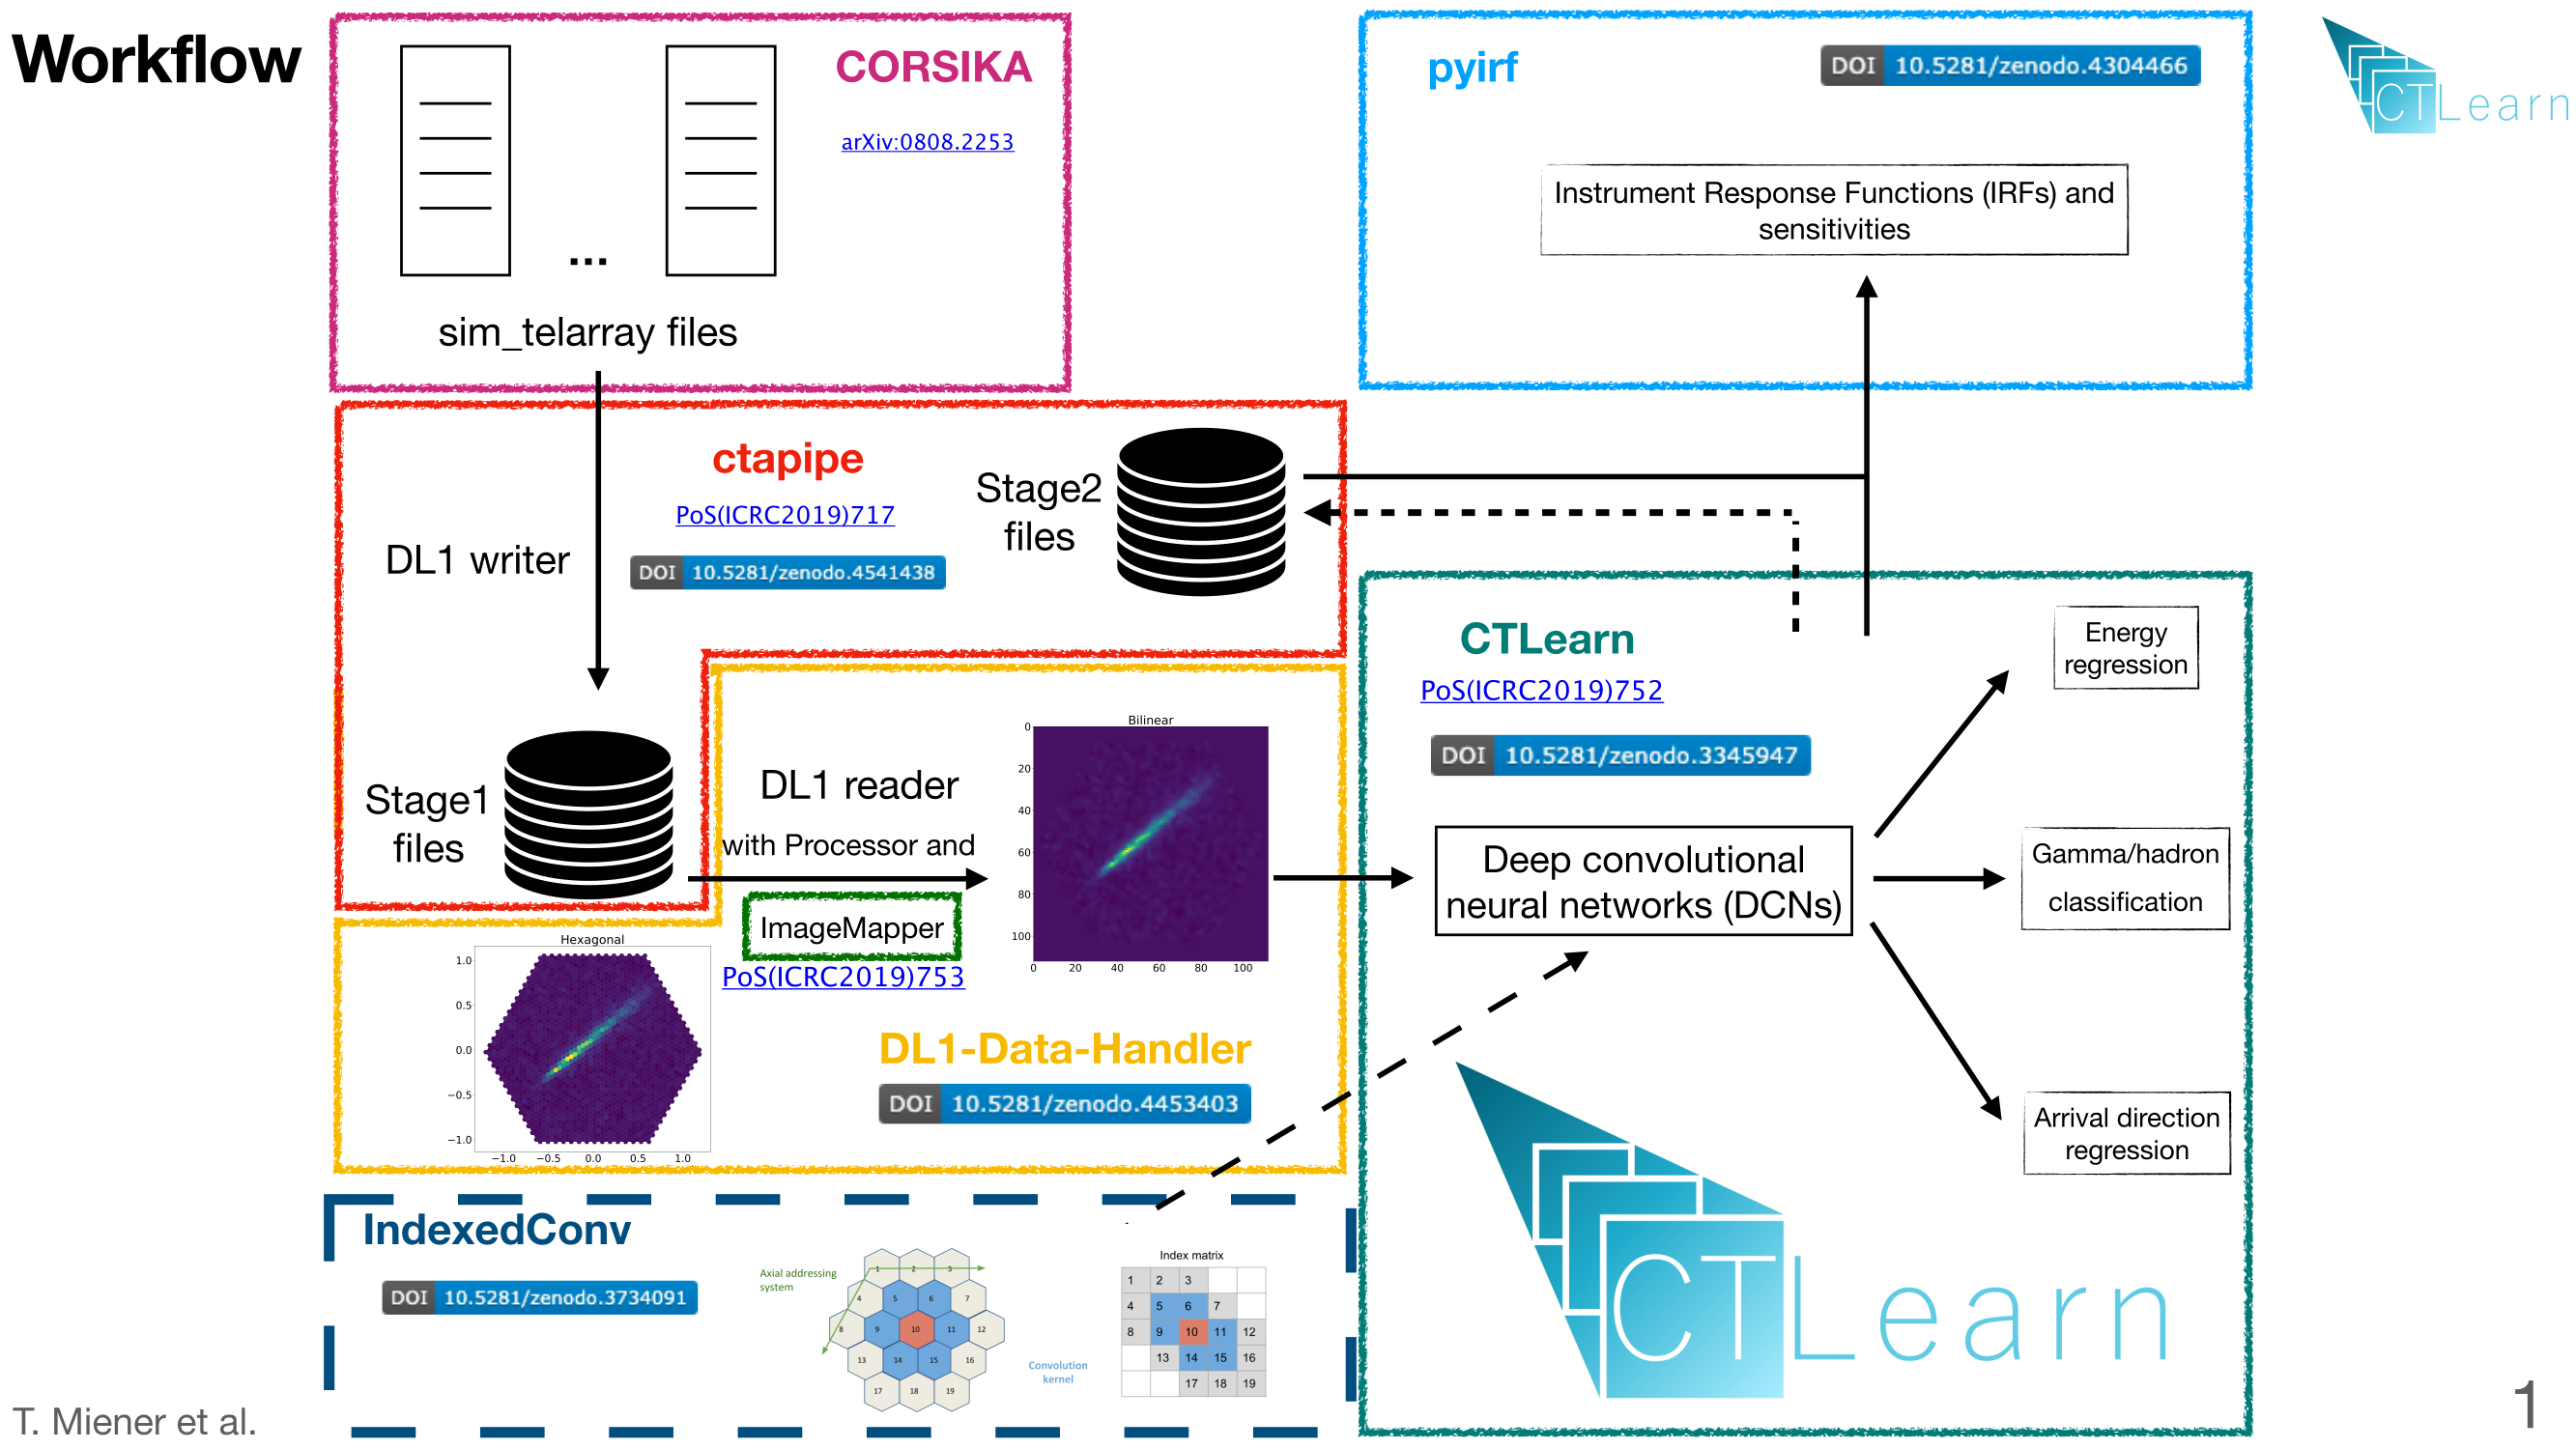
\includegraphics[width=0.6\linewidth]{ctlearnworkflow.png}
% 	\caption[Workflow CTLearn]{Workflow CTLearn. Source : \cite{CTLearn}}
% \end{figure}

% \section{Suite du travail}
% Ce projet de semestre en l'état a prouvé un intérêt pour une étape de prétraitement par pixel pour tout type d'\gls{iact} et pour de futurs télescopes spatiaux.
% Il a aussi été possible de déterminer les éléments nécessaires pour une possible utilisation de cette étape de prétraitement :
% \begin{itemize}
%     \item Établir un ou plusieurs métriques, ceci afin de pouvoir quantifier les améliorations ou régressions dues à des changements du modèle.
%     \item Établir un banc de test plus complet prenant en compte des facteurs externes comme la dégradation de capteurs ou autre.
%     \item Intégrer le modèle dans le simulateur CTLearn pour possiblement en améliorer ses performances et prouver une utilité pour des \gls{iact} terrestres.
% \end{itemize}
%%%%%%%%%%%%%%%%%%%%%%%%%%%%%%%